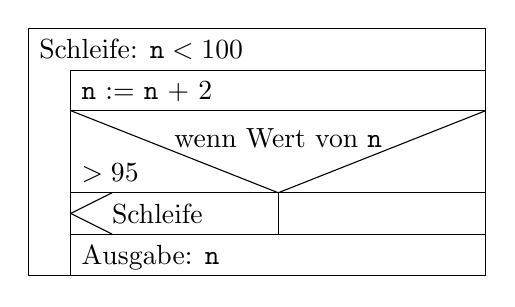
\begin{tikzpicture}
    \draw (0pt,0pt) rectangle (165.33552pt, -89.33958pt);
    \node at (4.0pt, -44.66979pt) {};
    \node at (40.79164pt, -7.6677100000000005pt) {Schleife: $\texttt{n} < 100$};
    \draw (15.33542pt,-15.33542pt) rectangle (165.33552pt, -29.77986pt);
    \node at (42.918735pt, -22.974304999999998pt) {\texttt{n} := \texttt{n} + 2};
    \draw (15.33542pt,-29.77986pt) rectangle (165.33552pt, -59.4507pt);
    \node at (19.33542pt, -44.61528pt) {};
    \draw (15.33542pt, -29.77986pt) -- (90.33547pt, -59.4507pt);
    \draw (90.33547pt, -59.4507pt) -- (165.33552pt, -29.77986pt);
    \node at (29.61319pt, -52.42397pt) {$> 95$};
    \node at (161.33552pt, -55.4507pt) {};
    \node at (90.33547pt, -39.670139999999996pt) {wenn Wert von \texttt{n}};
    \draw (15.33542pt,-59.4507pt) rectangle (90.33547pt, -74.39514pt);
    \node at (19.33542pt, -66.92292pt) {};
    \node at (46.668775pt, -66.92292pt) {Schleife};
    \draw (30.27986pt, -59.4507pt) -- (15.33542pt, -66.92292pt);
    \draw (15.33542pt, -66.92292pt) -- (30.27986pt, -74.39514pt);
    \draw (90.33547pt,-59.4507pt) rectangle (165.33552pt, -74.39514pt);
    \node at (94.33547pt, -66.92292pt) {};
    \draw (15.33542pt,-74.39514pt) rectangle (165.33552pt, -89.33958pt);
    \node at (44.210445pt, -82.83957999999998pt) {Ausgabe: \texttt{n}};
\end{tikzpicture}
